\documentclass[HARVARD,Utopia2COL]{WileyNJDv5}

\usepackage{amsmath,amssymb,booktabs}
\usepackage{graphicx}
\hypersetup{hidelinks}

\articletype{Research Article}
\journal{Journal of Futures Markets}
\raggedbottom

\begin{document}

\title{When Does Posterior Integration Change Option Values? Evidence from WTI Average Price Options}

\author[1]{Heriberto Espino Montelongo}
\authormark{ESPINO MONTELONGO}
\titlemark{POSTERIOR INTEGRATION IN WTI AVERAGE PRICE OPTIONS}

\address[1]{\orgname{Universidad de las Am\'ericas Puebla}, \orgaddress{\state{Puebla}, \country{Mexico}}}
\corres{Corresponding author: Heriberto Espino Montelongo. \email{[corresponding email]}}

\abstract[Abstract]{
This paper asks when integrating posterior uncertainty in historically estimated volatility materially changes a WTI Average Price Option value, and how that effect compares with changing the volatility input itself. Under the maintained one-factor pricing map, the posterior-integrated minus posterior-mean correction is governed locally by posterior variance and price curvature. A 175,000-history synthetic experiment confirms this mechanism and identifies weak-information, high-curvature states in which the correction can become economically relevant. In the observed October-2026 WTI panel, however, the mean absolute correction is 0.000745 while the mean width of the 95\% posterior model-price interval is 0.2733: a small change in the posterior mean price does not imply negligible parameter-induced price uncertainty. In 2,381 strict forward-in-time holdouts, prior option-implied volatility inputs sharply outperform the tested historical-volatility inputs. Rolling-window, exponentially weighted, and horizon-matched GARCH benchmarks do not reproduce that performance, and same-contract prior-IV carry shows that the improvement is not contingent on flexible smile fitting. An independent vanilla-WTI option surface provides a cross-instrument confirmation. The evidence therefore supports a diagnostic distinction: posterior integration can matter through curvature, but in this sample volatility-input choice is the larger empirical pricing margin.
}

\keywords{Bayesian option pricing; Asian options; WTI crude oil; parameter uncertainty; commodity derivatives}

\maketitle


\section{Introduction}\label{sec:introduction}

Option values depend on parameters and state variables that are estimated rather than observed. A Bayesian treatment can propagate that uncertainty through the pricing map instead of collapsing it to a single estimate. This idea is established in option pricing: Bayesian learning has been used in implied-volatility forecasting \cite{guidolin2003}, risk-neutral predictive densities \cite{romboutsstentoft2014}, and calibration of exotic-derivative models \cite{guptareisinger2014}. The narrower question studied here is when posterior integration itself materially changes a point price relative to plugging in the posterior mean of volatility.

Average-price commodity options are a useful setting because the pricing map depends on moneyness, maturity, and the fraction of the averaging window already fixed. The numerical literature exploits geometric-average structure to price arithmetic-average claims efficiently \cite{kemnavorst1990,curran1994}, while commodity-specific models allow richer futures dynamics \cite{schwartz1997,ewaldwu2023}. For WTI specifically, \cite{shirayatakahashi2011} calibrate richer risk-neutral models to liquid vanilla options before valuing average-price options, and \cite{ganwangyang2020} study WTI Average Price Options with a model-free machine-learning approach. The contribution here is therefore not a new APO pricing model. It is a diagnostic comparison between posterior integration and volatility-input choice under a deliberately transparent benchmark.

The statistical and pricing measures are kept separate. Historical returns inform volatility under the physical measure, while option valuation is performed under the risk-neutral measure. Let \(C^Q(\sigma)\) denote the risk-neutral APO value conditional on volatility \(\sigma\). The posterior-integrated and posterior-mean rules are
\begin{equation}
 C_{PI}=\mathbb E[C^Q(\sigma)\mid\mathcal D],
 \qquad
 C_{PM}=C^Q(\mathbb E[\sigma\mid\mathcal D]).
 \label{eq:intro_rules}
\end{equation}
Because \(C^Q(\sigma)\) is nonlinear, these quantities need not coincide. A second-order expansion gives
\begin{equation}
 C_{PI}-C_{PM}
 \approx
 \frac12 C^{Q\prime\prime}(\bar\sigma)
 \operatorname{Var}(\sigma\mid\mathcal D),
 \qquad
 \bar\sigma=\mathbb E[\sigma\mid\mathcal D].
 \label{eq:intro_taylor}
\end{equation}
The mechanism is therefore simple: posterior integration matters when posterior dispersion meets pricing curvature. By contrast, the width of the posterior distribution of model prices is first-order in posterior standard deviation, so a small \(C_{PI}-C_{PM}\) need not imply little parameter-induced price uncertainty.

The empirical application uses CME WTI Average Price Options. The payoff depends on the arithmetic average of daily first-nearby WTI futures settlements, so valuation reconstructs realized fixings, the remaining first-nearby futures sequence, and the contemporaneous futures curve. The observed option panel is then used in three complementary exercises. First, a synthetic mechanism map isolates the conditions under which posterior integration becomes economically relevant. Second, strict forward-in-time APO experiments compare historical-volatility inputs with volatility states inferred only from earlier option observations. Third, an independent validation constructs the volatility state from standard monthly WTI futures options rather than from the APO family itself.

The empirical distinction between integration and specification is important because option-implied information can outperform historical return models even when the pricing model remains imperfect. Forward-looking crude-oil option information has been shown to contain predictive volatility content beyond historical models \cite{gildertsiaras2020}, and flexible implied-volatility specifications can fit the contemporaneous cross-section while still deteriorating out of sample \cite{dumasflemingwhaley1998}. More generally, richer option models can improve some performance criteria without dominating on all dimensions \cite{bakshicaochen1997,cumminsesposito2025}. The paper therefore treats an implied volatility as an effective state under the maintained pricing map, not as a structural estimate of a unique risk-neutral diffusion coefficient.

Three findings organize the paper. First, the synthetic experiments confirm Equation~\eqref{eq:intro_taylor}: the PI--PM correction grows with posterior dispersion and volatility curvature and can become material in weak-information, high-volatility, long-horizon states. Second, the observed WTI panel lies in a region where the mean-price correction is very small even though the posterior distribution of theoretical prices remains meaningfully dispersed. Third, changing the volatility information supplied to the model has a much larger empirical effect. Prior option-implied states sharply reduce settlement pricing error relative to the historical-volatility benchmarks evaluated here; this result survives recent-window, EWMA, and horizon-matched GARCH comparisons, does not require flexible smile fitting, and persists when the volatility source is moved to an independent vanilla-WTI option market.

These findings do not identify a pure structural wedge between physical and risk-neutral volatility. Option-implied states can absorb risk premia, stochastic volatility, jumps, omitted futures-curve dynamics, liquidity, and settlement-marking effects. The supported conclusion is narrower: in this sample, prior option-implied volatility states are substantially more informative for subsequent APO settlements than the tested historical-volatility inputs, while more exact integration of the historical-volatility posterior changes the point-price mean much less.

The rest of the paper gives each finding one principal home. Section~\ref{sec:contract} describes the contract and data. Section~\ref{sec:methodology} combines the statistical, pricing, and validation design. Section~\ref{sec:results} reports the mechanism and market evidence. Section~\ref{sec:robustness} summarizes robustness checks, with detailed implementation and diagnostics moved to the online supplement. Section~\ref{sec:conclusion} concludes.

\section{WTI Average Price Options and the empirical setting}\label{sec:contract}

\subsection{Contract mechanics}

CME WTI Average Price Options are cash-settled options whose payoff is linked to the arithmetic average of daily settlements of first-nearby WTI crude-oil futures during the relevant calendar month. For an averaging month with fixing dates $t_1,\ldots,t_M$, define
\begin{equation}
 A_T=\frac{1}{M}\sum_{j=1}^{M}F^{(1)}_{t_j},
 \label{eq:apo_average}
\end{equation}
where $F^{(1)}_{t_j}$ denotes the settlement of the first-nearby CL futures contract applicable to fixing date $t_j$. A call and put have terminal payoffs
\begin{align}
 H_C&=(A_T-K)^+,\\
 H_P&=(K-A_T)^+.
\end{align}
The first-nearby designation matters because the futures contract contributing to the average can change during the averaging period. The payoff is therefore not, in general, an average of repeated observations of one fixed futures maturity. This contract feature is also explicit in the WTI average-option treatment of \cite{shirayatakahashi2011}, where two consecutive WTI futures maturities enter the monthly averaging window because the nearby futures contract expires before month-end.

At an option valuation date $t$ inside the averaging month, let $\mathcal R_t$ denote fixing dates already realized and $\mathcal U_t$ the remaining fixing dates. The final average can be decomposed as
\begin{equation}
 A_T=\frac{1}{M}
 \left(
 \sum_{j\in\mathcal R_t}F^{(1)}_{t_j}
 +
 \sum_{j\in\mathcal U_t}F^{(1)}_{t_j}
 \right).
 \label{eq:partial_fixing}
\end{equation}
This decomposition is central to the empirical pricing exercise. Realized fixings are known constants; only the remaining components are simulated under the risk-neutral measure. As the averaging month progresses, the option mechanically loses exposure to future volatility because a larger share of $A_T$ has already been fixed.

A useful state variable for cross-sectional analysis is the risk-neutral expected final average,
\begin{equation}
 \widehat A^{Q}_{t,T}=
 \frac{1}{M}
 \left(
 \sum_{j\in\mathcal R_t}F^{(1)}_{t_j}
 +
 \sum_{j\in\mathcal U_t}\mathbb E_t^Q[F^{(1)}_{t_j}]
 \right).
 \label{eq:expected_average}
\end{equation}
We define log moneyness observation by observation as
\begin{equation}
 m_{t,K,T}=\log\!\left(\frac{K}{\widehat A^{Q}_{t,T}}\right).
 \label{eq:moneyness}
\end{equation}
For calls, negative values correspond to strikes below the expected average; for puts the economic interpretation is reversed in terms of intrinsic direction. This measure is preferable to assigning a contract a fixed moneyness category using the futures price on the final sample date.

\subsection{Why WTI is informative for parameter uncertainty}

WTI provides a demanding empirical environment for the question studied in this paper. Oil prices can exhibit rapid changes in level, realized volatility, and the shape of the futures curve. These changes imply that the same option can move through substantially different moneyness states during its observed history. They also create episodes in which a posterior estimated from a shorter historical window is more dispersed than one estimated from a long sample.

The analysis does not attribute individual price moves mechanically to geopolitical events. Such causal statements would require a separate event-study design. Instead, the paper conditions its claims on observed return histories, posterior dispersion, option state variables, and the market-implied volatility information available before each valuation date.

\subsection{Barchart option histories}

The empirical database was assembled from individual Barchart historical series for WTI Average Price Options. The use of Barchart WTI APO observations has an empirical precedent in \cite{ganwangyang2020}, who apply a model-free deep-learning approach to WTI average-option pricing; the present study instead uses the data to evaluate a structural physical/risk-neutral decomposition and posterior-integration mechanism. The downloaded maturities are September 2026, October 2026, November 2026, March 2027, September 2027, March 2028, September 2028, and June 2029. Calls and puts were retained as available. Rather than choosing only contracts that appear near the money on one date, the raw panel keeps all downloaded contracts and lets moneyness vary by date according to Equation~\eqref{eq:moneyness}.

The ingestion pipeline recursively audits the raw CSV directory, parses option symbols, derives strike and option type, checks the symbol-implied expiry against the storage folder, and de-duplicates contracts before constructing the option-date panel. The current audit identifies 214 input files, 213 unique contracts, and 11,179 option-date observations. One file is stored under a folder inconsistent with its symbol-implied expiry; the parser records the mismatch and uses the contract symbol rather than silently trusting the directory name.

The histories contain end-of-day fields including open, high, low, latest, volume, and open interest. In the source histories used for this study, Barchart \texttt{Latest} is the end-of-day settlement field. At least one contract/date comparison also reproduces the corresponding CME daily settlement exactly. The field is therefore used as the market settlement benchmark, while the paper stops short of claiming that the full proprietary panel has been independently reconciled observation by observation against official CME bulletins. This distinction matters because many histories contain zero reported volume while open interest remains positive.

Liquidity is consequently used as a diagnostic and robustness dimension rather than a binary requirement that every observation have positive trading volume. Results are reported for the full eligible panel, positive-volume subsets, and multiple open-interest thresholds. Contracts with sparse trading can still contain an exchange settlement, but conclusions that depend exclusively on such observations are treated cautiously.

The data pipeline also produces a variable called \texttt{richest}, inherited from an earlier data-audit routine. It measures information completeness using the number of sessions, calendar span, and field completeness. It does \emph{not} measure liquidity, trading intensity, or economic importance. The variable is retained for data-quality diagnostics but is not used as the economic contract-selection rule.

\subsection{Independent vanilla-WTI option data}

The external risk-neutral validation uses standard monthly American WTI options on futures (CME product LO) obtained through Databento's CME Globex historical service. The required market objects are official LO option settlements, matching CL futures settlements, and the instrument definitions needed to recover strike, option type, underlying futures contract, and expiration. Raw vendor records are treated as proprietary inputs and are not redistributed.

For the October-2026 validation, the final vanilla sample uses LO options written on CLX6 and CLZ6 with strikes from 70 to 120 over trading reference dates from August 24 through September 10, 2026. The acquisition window is chosen to precede the APO target dates used in the strict external test. The final inversion panel contains 5,220 successful contract-date implied volatilities over 13 reference dates; 5,214 underlying option settlements are flagged actual and six theoretical. These observations are used only to construct the external volatility state described in Section~\ref{sec:external_lo_method}; APO prices never enter that inversion.

\subsection{Maturity coverage}

The chosen expiries deliberately span the maturity dimension rather than concentrating exclusively on consecutive nearby months. The first three maturities provide short-horizon contracts, while March 2027 through June 2029 extend the cross section toward medium and long horizons. This structure is useful because Equation~\eqref{eq:intro_taylor} predicts that the importance of posterior uncertainty depends not only on posterior dispersion but also on the curvature of the pricing map, which can change materially with time to maturity.

The number of available strikes and the depth of trading are not constant across maturities. In particular, the far end of the curve contains fewer contracts. The empirical design does not force a balanced panel. Instead, it preserves the observed contract set and treats maturity coverage, liquidity, and availability of matching CL futures histories as explicit scope constraints.

\section{Methodology and research design}\label{sec:methodology}\label{sec:design}

\subsection{Physical inference and risk-neutral pricing}

Historical WTI returns are modeled under the physical measure with a constant-volatility geometric Brownian motion. For log return \(R_i\) over interval \(\Delta t\),
\begin{equation}
 R_i\sim
 \mathcal N\!\left[
 \left(\mu-\frac12\sigma^2\right)\Delta t,
 \sigma^2\Delta t
 \right].
 \label{eq:return_likelihood}
\end{equation}
The baseline prior is
\begin{equation}
 \mu\sim\mathcal N(0,1),
 \qquad
 \sigma\sim\operatorname{InvGamma}(2,0.1),
 \quad \sigma>0.
 \label{eq:priors}
\end{equation}
Posterior sampling uses a random-walk Metropolis algorithm in \((\mu,\log\sigma)\). The large synthetic experiments additionally integrate \(\mu\) analytically conditional on \(\sigma\), producing a one-dimensional deterministic posterior calculation that is independent of MCMC error. The detailed sampler settings, calibration checks, and sensitivity specifications are reported in the online supplement.

Valuation is performed separately under the risk-neutral measure. For each unresolved WTI fixing, the maintained futures benchmark is
\begin{equation}
 dF_u=\sigma F_u\,dW_u^Q.
 \label{eq:futures_q}
\end{equation}
The historical drift does not enter the pricing dynamics. Realized fixings enter the arithmetic average deterministically; only future first-nearby settlements remain stochastic. Each remaining fixing is initialized from the corresponding point of the observed CL futures curve rather than from one fixed futures contract. This representation is deliberately simple so that posterior integration can be isolated from richer commodity dynamics.

Baseline empirical prices are computed by Monte Carlo. Curran conditioning \cite{curran1994} provides a deterministic implementation of the same one-factor pricing map and is used for large forward comparisons and sensitivity calculations. Difficult contracts are also checked with high-precision pseudo-random and scrambled-Sobol calculations. Numerical diagnostics are summarized in Section~\ref{sec:robustness} and documented in detail in the supplement.

\subsection{Posterior integration and model-price uncertainty}

The primary comparison is between
\begin{equation}
 C_{PI}=\mathbb E[C^Q(\sigma)\mid\mathcal D],
 \qquad
 C_{PM}=C^Q(\bar\sigma),
 \qquad
 \bar\sigma=\mathbb E[\sigma\mid\mathcal D].
 \label{eq:estimators}
\end{equation}
A Taylor expansion around \(\bar\sigma\) gives the central mechanism,
\begin{equation}
 C_{PI}-C_{PM}
 \approx
 \frac12 C^{Q\prime\prime}(\bar\sigma)
 \operatorname{Var}(\sigma\mid\mathcal D).
 \label{eq:taylor_gap}
\end{equation}
The mean-price correction is therefore locally second order in posterior dispersion. By contrast,
\begin{equation}
 \operatorname{SD}\!\left(C^Q(\sigma)\mid\mathcal D\right)
 \approx
 |C^{Q\prime}(\bar\sigma)|
 \sqrt{\operatorname{Var}(\sigma\mid\mathcal D)},
 \label{eq:price_uncertainty_delta}
\end{equation}
so posterior model-price uncertainty is locally first order in posterior standard deviation. These are distinct objects: close posterior-integrated and posterior-mean point prices do not imply a narrow posterior distribution of theoretical prices.

The paper also reports posterior-mode and likelihood plug-ins in the repeated-sampling benchmark, but they are secondary to the PI--PM comparison. A posterior-RMS volatility is used only as a scalar sensitivity check; it is not treated as an alternative Bayesian integration rule.

\subsection{Synthetic mechanism experiment}

Synthetic return histories are generated under \(\mathbb P\), while target option values are evaluated under \(\mathbb Q\) at the known data-generating volatility. The large mechanism map contains 175,000 independent histories and spans short to long estimation samples, annual volatility from 0.10 to 0.80, multiple maturities and moneyness states, and partial-fixing configurations. For each history and contract state, the experiment records the PI--PM gap, posterior variance of volatility, local pricing curvature, and the approximation in Equation~\eqref{eq:taylor_gap}.

The purpose is not to optimize a pricing method against market data. It is to identify the state variables under which posterior integration becomes economically relevant and to test whether the curvature--dispersion approximation explains the observed gap. Exact grids and replication counts by cell are retained in the online supplement.

\subsection{Forward WTI APO validation}

The empirical design uses only information available by each valuation date. Historical-volatility posteriors are estimated from expanding return histories with no future returns. APO-implied effective volatilities are obtained by inverting the same Curran pricing map contract by contract and are interpreted as model-equivalent risk-neutral states, not structural diffusion coefficients.

The principal predictive experiment estimates APO volatility surfaces only from dates strictly earlier than the target date. A previous-day specification uses the latest completed earlier date, while an expanding specification pools earlier dates with recency weights. Seven expiries pass the committed-data coverage rule, producing 2,381 strict forward-in-time contract-date holdouts over 15 target dates.

Two benchmark families probe competing explanations for the option-informed result. First, historical information is made more recent through 63-, 126-, and 252-return realized-volatility windows, a 63-business-day half-life EWMA, and a Gaussian GARCH(1,1) conditional-variance forecast mapped to each APO's remaining fixing horizon. These are benchmark forecasts under the same pricing representation, not alternative risk-neutral structural models. Second, a same-contract persistence rule carries the latest strictly prior APO implied volatility forward and reprices the contract using its target-date futures curve, discount factor, realized fixings, and remaining schedule. This isolates whether the predictive gain requires a flexible cross-sectional smile. Detailed GARCH construction and scalar-matching formulas are moved to the supplement.

Pricing errors are measured against end-of-day option settlements using mean error, MAE, and RMSE. Because contracts observed on the same date share the market state and futures curve, uncertainty comparisons are resampled by valuation-date cluster rather than by individual option row. Liquidity restrictions based on positive volume and open interest are reported as robustness checks.

\subsection{Independent vanilla-WTI validation}\label{sec:external_lo_method}

The APO experiment remains within the same option family used as the pricing target. An independent validation therefore derives the volatility state from standard monthly American WTI futures options (CME product LO). Official LO settlements are matched to their CL futures settlements and inverted with an American Cox--Ross--Rubinstein futures-option tree. The production inversion uses 160 tree steps; refinement diagnostics are reported in the supplement.

For each APO target date, every LO observation used to construct the external volatility surface is strictly earlier than the target. Surfaces are fitted separately by underlying futures contract and evaluated at the target APO strike. The maturity-specific LO volatilities are then mapped into the maintained scalar-volatility APO engine. The primary mapping is a fixing-count weighted RMS rule; a separate sensitivity chooses the scalar volatility that matches the unresolved arithmetic-average variance under the same common-factor representation. The purpose of this sensitivity is to test the transfer rule, not to claim that either scalar is an exact structural representation.

The primary external comparison is restricted to APO observations lying inside the observed prior LO moneyness support for both external specifications. This yields 253 common-support contract-dates over 10 target dates. Same-day APO prices never enter the external volatility construction. The experiment therefore asks whether the option-informed pricing advantage survives when the volatility source is moved outside the APO family.

\subsection{Scope of supporting diagnostics}

Several checks are deliberately kept outside the main evidentiary flow: prior and estimation-window sensitivity, Student-\(t\) physical returns, contract-reconstructed first-nearby return histories, posterior-RMS plug-in pricing, simulation-based calibration, detailed Monte Carlo/Sobol/Curran comparisons, LO tree refinement, surface-shape diagnostics, and full liquidity tables. Section~\ref{sec:robustness} reports only what these checks establish for the three central findings; implementation settings and complete numerical results are preserved in the online supplement.

\section{Results}\label{sec:results}

The completed evidence separates four questions. First, when does posterior integration differ materially from posterior-mean plug-in pricing? Second, can a small PI--PM mean correction coexist with substantial posterior model-price dispersion? Third, how large is the integration effect relative to changing the volatility input, including stronger recent-history and persistence benchmarks? Fourth, does the option-informed result survive when the volatility state comes from an independent vanilla-WTI market?

\subsection{Repeated-sampling benchmark}

Table~\ref{tab:synthetic_pilot} reports the original repeated-sampling benchmark. Even with only 63 daily observations, posterior-integrated and posterior-mean plug-in pricing are nearly indistinguishable. As the historical sample increases, all four estimators converge and the PI--PM difference becomes numerically negligible.

\begin{table*}[t]
\centering
\caption{Repeated-sampling point-pricing performance. The target is the risk-neutral price evaluated at the true volatility, not a posterior-generated target. The sigma-mode comparator is the marginal posterior mode of volatility rather than a joint MAP estimate. Posterior interval coverage is reported separately in the text because the interval procedure is common across point estimators.}\label{tab:synthetic_pilot}
\begin{tabular}{llrrr}
\toprule
$N$ & Method & Bias & MAE & RMSE\\
\midrule
63 & Posterior-integrated & -0.0011 & 0.3543 & 0.4686\\
63 & Posterior-mean plug-in & -0.0012 & 0.3543 & 0.4687\\
63 & Sigma posterior-mode plug-in & -0.0919 & 0.3783 & 0.4867\\
63 & MLE plug-in & -0.0407 & 0.3576 & 0.4701\\
\addlinespace
252 & Posterior-integrated & 0.0139 & 0.1988 & 0.2454\\
252 & Posterior-mean plug-in & 0.0139 & 0.1988 & 0.2454\\
252 & Sigma posterior-mode plug-in & -0.0212 & 0.1974 & 0.2446\\
252 & MLE plug-in & 0.0035 & 0.1992 & 0.2444\\
\addlinespace
1260 & Posterior-integrated & -0.0048 & 0.1010 & 0.1243\\
1260 & Posterior-mean plug-in & -0.0048 & 0.1010 & 0.1243\\
1260 & Sigma posterior-mode plug-in & -0.0128 & 0.1060 & 0.1302\\
1260 & MLE plug-in & -0.0067 & 0.1013 & 0.1243\\
\bottomrule
\end{tabular}
\end{table*}

The central 95\% posterior model-price interval has empirical coverage 0.9500, 0.9625, and 0.9250 for $N=63,252,$ and $1260$, respectively. These are properties of the posterior interval procedure and are not separate coverage statistics for each point estimator.

The near equality of $\widehat C_{PI}$ and $\widehat C_{PM}$ is not a generic Bayesian result. It is a property of the posterior dispersion and pricing curvature in these particular states. The massive mechanism experiment makes this distinction explicit.

\subsection{Where posterior integration matters}

The mechanism map covers 175,000 independently simulated historical datasets and 168 WTI-like contract states. Across the complete experiment, the largest observed absolute PI--PM gap is 0.1384. The largest cell-level 99th percentile is 0.1271. These values are orders of magnitude larger than the roughly $10^{-3}$ gaps observed in the WTI baseline, so the empirical near-equivalence of PI and PM is not an artifact of a pricing rule that can never separate.

The mechanism map normalizes the WTI-like forward level to \$100 per barrel, so the maximum gap of 0.1384 is \$0.1384 per barrel. Under the WTI APO contract multiplier of 1,000 barrels and ordinary minimum price fluctuation of \$0.01 per barrel, that scale corresponds to approximately \$138.40 per contract, or 13.84 ordinary ticks \cite{cme_wti_apo_rule}. This conversion gives the synthetic separation an explicit economic scale; it does not imply that every state attaining the statistical maximum would be equally tradable.

The adverse states have a clear economic structure. The largest gaps occur with short historical samples, high true volatility, long remaining horizons, little realized fixing, and strikes far from the expected average. For example, with $n=21$, $\sigma_0=0.80$, 126 days to maturity, no realized fixing, and moneyness 1.50, the mean PI--PM gap is 0.1176 and the 99th percentile is 0.1271. With $n=21$, $\sigma_0=0.50$, 252 days, no realized fixing, and moneyness 1.50, the mean gap is 0.1103 and the maximum observed gap is 0.1384.

The mechanism in Equation~\eqref{eq:taylor_gap} explains these states remarkably well. In the most adverse cells, the correlation between the realized PI--PM gap and the second-order approximation is approximately 0.999, with through-origin slopes close to one. Posterior dispersion also behaves as expected: for $\sigma_0=0.80$, mean posterior standard deviation falls from approximately 0.122 at $n=21$ to 0.0159 at $n=1260$. The experiment therefore turns the qualitative Jensen argument into a quantitative state map: integration matters when \emph{both} posterior dispersion and price curvature are large.

Partial fixing works in the opposite direction. As a larger fraction of the final arithmetic average becomes deterministic, the remaining volatility exposure shrinks and so does the opportunity for posterior integration to change the point price. This effect is visible even in high-volatility, extreme-moneyness cells and provides a contract-specific reason why parameter uncertainty can matter early in an averaging problem but fade rapidly as fixings accumulate.

Figure~\ref{fig:mechanism_map} condenses these mechanism results. Panel A shows posterior dispersion shrinking with historical information; Panels B and C show how the integration gap grows in high-curvature, weakly fixed states and then contracts as fixings accumulate; Panel D compares the realized PI--PM gap with the second-order approximation across the complete synthetic state map.

\begin{figure*}[t]
\centering
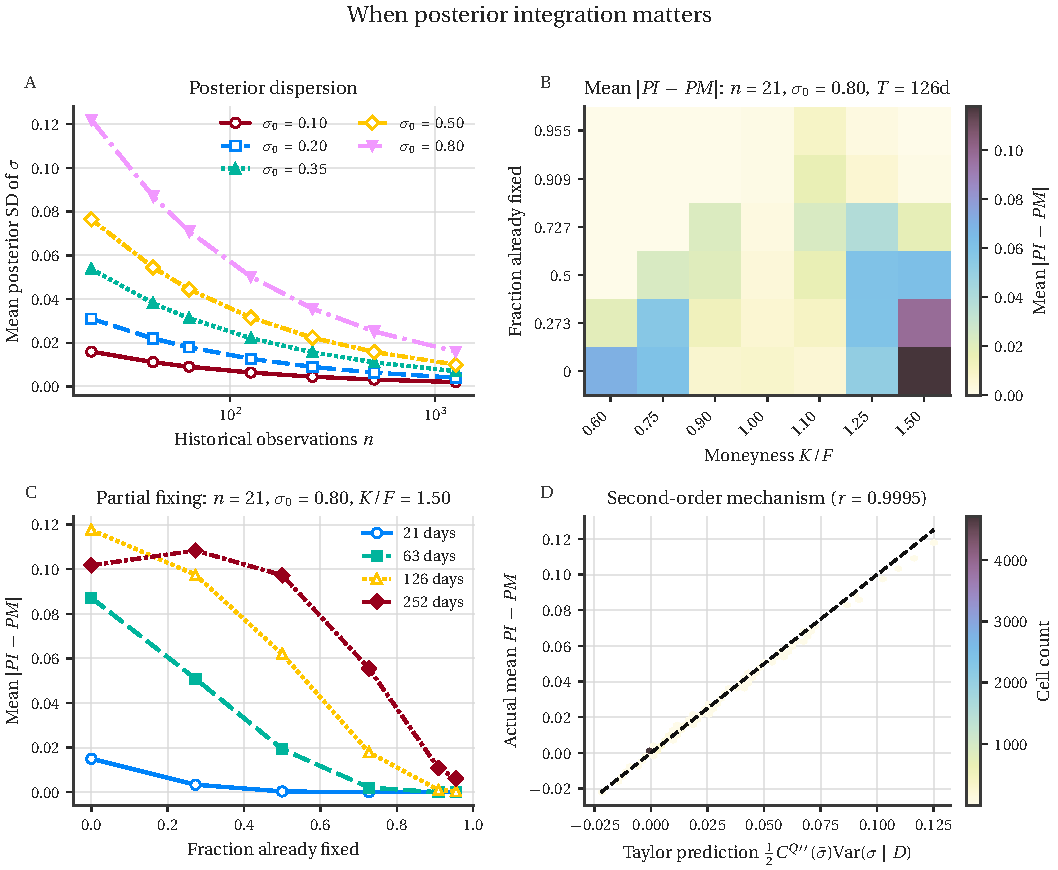
\includegraphics[width=\textwidth]{figures/publication/fig01_mechanism_map.pdf}
\caption{Mechanism map for posterior integration. Panel A reports the mean posterior standard deviation of $\sigma$ against historical sample size for the simulated volatility levels. Panel B shows mean $|PI-PM|$ across moneyness and partial-fixing states for $n=21$, $\sigma_0=0.80$, and 126 days to maturity. Panel C traces the same integration gap against the fraction already fixed at $K/F=1.50$ for the four maturity horizons. Panel D compares the actual cell-level mean PI--PM gap with the second-order Taylor term in Equation~\eqref{eq:taylor_gap}; the correlation across synthetic cells is 0.9995. The figure uses only independently simulated histories and prices under the maintained one-factor risk-neutral map.}
\label{fig:mechanism_map}
\end{figure*}

\subsection{Contract-consistent October-2026 baseline}

The first completed WTI baseline uses the October-2026 APO expiry. Across 12 eligible valuation dates, the main sample contains 310 option-date observations. Five dates contain at least one positive-volume contract, producing a 136-observation positive-volume-date sample, while only six individual contract-date observations themselves report positive daily volume.

Table~\ref{tab:oct26_empirical} reports pooled model-to-market errors. All rules use the same futures curves, realized fixings, discount factors, and market settlements; the comparison therefore isolates the incremental effect of the volatility decision rule within the maintained model.

\begin{table*}[t]
\centering
\caption{October-2026 WTI APO point-pricing errors and posterior price uncertainty. Mean error is model price minus the Barchart end-of-day settlement field. Panel B compares the nonlinear PI--PM mean-price correction with the width of the central 95\% posterior distribution of theoretical prices.}\label{tab:oct26_empirical}

\textit{Panel A: point-pricing errors}\\[2pt]
\begin{tabular}{llrrrr}
\toprule
Sample & Method & $N$ & Mean error & MAE & RMSE\\
\midrule
All eligible dates
 & Posterior-integrated & 310 & -0.4065 & 0.4079 & 0.5177\\
 & Posterior mean & 310 & -0.4072 & 0.4086 & 0.5183\\
 & Sigma posterior mode & 310 & -0.4122 & 0.4132 & 0.5200\\
 & MLE & 310 & -0.4088 & 0.4101 & 0.5197\\
\addlinespace
Positive-volume dates
 & Posterior-integrated & 136 & -0.3601 & 0.3633 & 0.4303\\
 & Posterior mean & 136 & -0.3609 & 0.3640 & 0.4310\\
 & Sigma posterior mode & 136 & -0.3697 & 0.3720 & 0.4413\\
 & MLE & 136 & -0.3625 & 0.3654 & 0.4324\\
\addlinespace
Positive-volume contracts
 & Posterior-integrated & 6 & -0.1388 & 0.1543 & 0.1864\\
 & Posterior mean & 6 & -0.1394 & 0.1547 & 0.1869\\
 & Sigma posterior mode & 6 & -0.1530 & 0.1651 & 0.2026\\
 & MLE & 6 & -0.1414 & 0.1560 & 0.1882\\
\bottomrule
\end{tabular}

\vspace{5pt}
\textit{Panel B: mean-price correction versus posterior price dispersion}\\[2pt]
\begin{tabular}{lrrrr}
\toprule
Sample & $N$ & Mean $|PI-PM|$ & Mean 95\% width & Width / gap\\
\midrule
All eligible dates & 310 & 0.000745 & 0.2733 & 366.7\\
Positive-volume dates & 136 & 0.000802 & 0.2695 & 336.1\\
Positive-volume contracts & 6 & 0.000591 & 0.3660 & 619.7\\
\bottomrule
\end{tabular}
\end{table*}

Posterior integration and the posterior-mean plug-in are extremely close in every sample, but Panel B shows why that fact must not be read as absence of parameter uncertainty. Across all 310 observations, the mean central 95\% posterior price-interval width is 0.2733, roughly 367 times the mean absolute PI--PM correction. Among the six positive-volume contracts, the corresponding ratio is about 620. The empirical conclusion is therefore specific: the nonlinear shift in the posterior \emph{mean} price is small under the observed posterior and contract states, while the posterior distribution of theoretical model prices remains visibly dispersed.

The sign of the model-to-market errors is equally important. All four historical-volatility rules underprice the option settlements on average. This common bias cannot be explained by choosing PI rather than PM because the two rules produce almost the same prices. It points instead toward a larger specification discrepancy.

Because the empirical PI--PM differences are sub-cent, Section~\ref{sec:numerical_robustness} subjects them to high-precision pseudo-random Monte Carlo, randomized Sobol, and Curran benchmarks. The three engines recover the same integration gap to a scale far smaller than the gap itself, so the near-equivalence is not a simulation-noise artifact.

\subsection{Historical versus APO-implied effective volatility}

The September--October APO cross-section provides 402 contract-date observations for implied-volatility inversion. All 402 settlements can be mapped to a finite implied volatility under the maintained Curran-equivalent one-factor model. The median historical posterior mean is 0.4155. By contrast, the median date-level common volatility calibrated to the complete APO cross-section is 0.4577, a median difference of 0.0425. Contract-level implied volatilities have a still higher median of 0.4835 because the cross section contains pronounced strike variation.

These values should not be interpreted as proof that the diffusion coefficient must differ between $\mathbb P$ and $\mathbb Q$. They are effective parameters required by the maintained pricing map. Their economic importance is that they expose a specification margin much larger than the PI--PM correction.

Figure~\ref{fig:historical_vs_apo_iv} shows this distinction at both the date and strike levels. The historical posterior mean remains comparatively stable, whereas the model-equivalent APO-implied state moves with valuation date and exhibits clear strike variation.

\begin{figure*}[t]
\centering
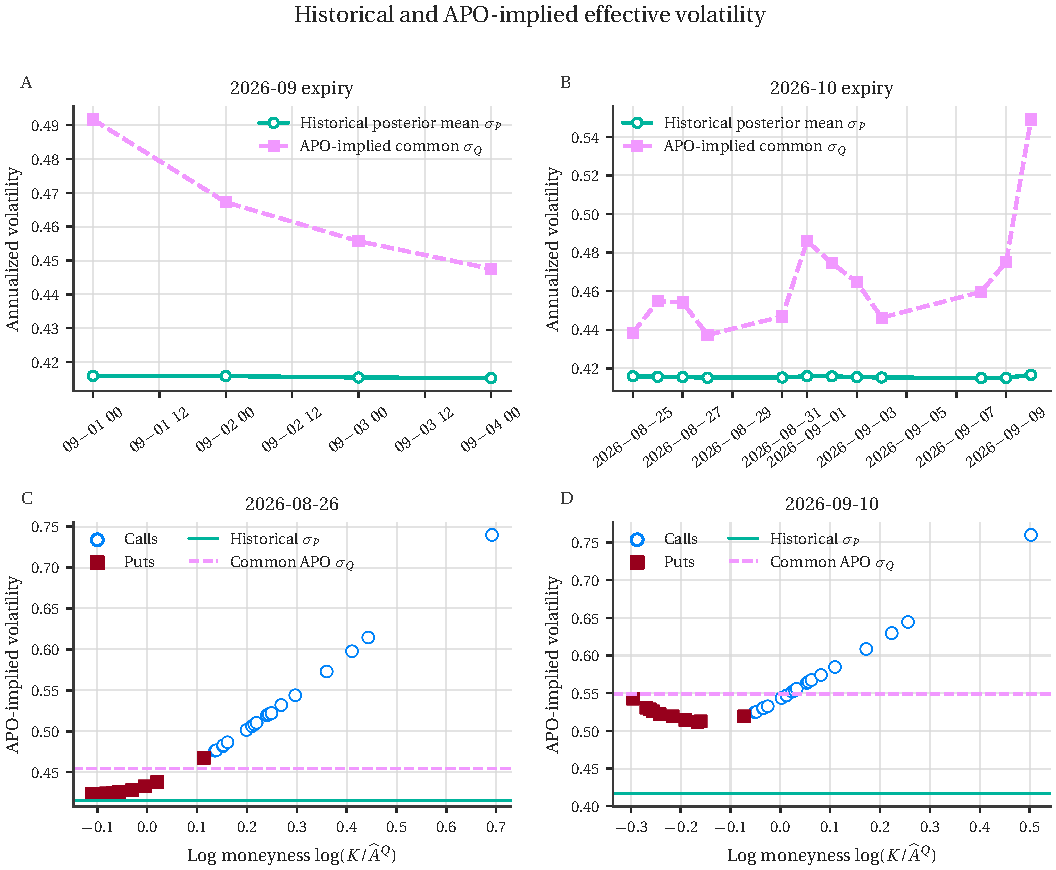
\includegraphics[width=\textwidth]{figures/publication/fig02_historical_vs_apo_implied_volatility.pdf}
\caption{Historical and APO-implied effective volatility in the September--October 2026 cross-section. Panels A and B compare the historical posterior mean $\sigma_P$ with the date-level common APO-implied $\sigma_Q$ for the September and October expiries. Panels C and D show contract-level APO-implied volatilities against log moneyness on August 26 and September 10, with horizontal references for the historical posterior mean and the date-level common APO-implied value. These implied volatilities are effective parameters under the maintained Curran-equivalent pricing map; they are not interpreted as unique structural diffusion coefficients.}
\label{fig:historical_vs_apo_iv}
\end{figure*}

Leave-one-contract-out calibration provides a first cross-sectional check. Across 399 targets, a common APO-calibrated volatility reduces MAE from 0.3450 for the historical-volatility PI baseline to 0.1557 and RMSE from 0.4625 to 0.1900. The improvement is not uniform, however. The nine positive-volume observations move in the opposite direction in aggregate, and cross-option-type transfer is weaker. These failures are consistent with the fact that one scalar volatility cannot reproduce the observed strike structure and that call/put samples occupy different moneyness regions.

\subsection{Strict forward-in-time volatility validation}

The stronger test predicts each target date using only implied-volatility observations from earlier dates. The extended experiment spans seven APO expiries from September 2026 through September 2028 and contains 2,381 holdout option-date observations. No same-day option settlement enters the fitted smile.

The extension reveals a pronounced term structure in the effective volatility required by the maintained pricing map. Median date-level common $\sigma_Q$ is 0.4478, 0.4572, and 0.4444 for the September, October, and November 2026 expiries, respectively; it then declines to 0.3609 for March 2027, 0.3001 for September 2027, 0.2647 for March 2028, and 0.2416 for September 2028. Over the same valuation dates, the historical posterior mean remains near 0.416. These $\sigma_Q$ values are model-equivalent parameters, not structural volatility estimates; the maturity pattern can absorb risk premia, smile effects, omitted futures-curve dynamics, and liquidity or marking effects.

Table~\ref{tab:forward_q} reports the corresponding strict-forward pricing errors by expiry.

\begin{table*}[t]
\centering
\caption{Strict forward-in-time APO volatility validation by expiry. The historical-volatility baseline is the posterior-integrated price from the canonical Monte Carlo engine on the same holdout observations. The prior-date APO volatility inputs are repriced with the deterministic Curran engine.}\label{tab:forward_q}
\begin{tabular}{lrrrrrrr}
\toprule
Expiry & $N$ & \multicolumn{3}{c}{MAE} & \multicolumn{3}{c}{RMSE}\\
\cmidrule(lr){3-5}\cmidrule(lr){6-8}
 & & Historical PI & Expanding & Previous day & Historical PI & Expanding & Previous day\\
\midrule
2026-09 & 198 & 0.1090 & 0.0433 & 0.0443 & 0.1378 & 0.0754 & 0.0695\\
2026-10 & 280 & 0.4159 & 0.1486 & 0.1543 & 0.5308 & 0.2772 & 0.2557\\
2026-11 & 285 & 0.4276 & 0.1653 & 0.1729 & 0.5267 & 0.2696 & 0.2548\\
2027-03 & 339 & 1.0599 & 0.1187 & 0.1070 & 1.0744 & 0.1560 & 0.1333\\
2027-09 & 429 & 2.8963 & 0.0789 & 0.0867 & 2.9324 & 0.0979 & 0.1012\\
2028-03 & 445 & 4.5398 & 0.1096 & 0.1022 & 4.5813 & 0.1392 & 0.1248\\
2028-09 & 405 & 5.8103 & 0.0962 & 0.0885 & 5.8979 & 0.1268 & 0.1152\\
\addlinespace
Pooled & 2,381 & 2.6187 & 0.1088 & 0.1075 & 3.4090 & 0.1725 & 0.1594\\
\bottomrule
\end{tabular}
\end{table*}

Figure~\ref{fig:forward_q_bootstrap} complements the point estimates with valuation-date cluster uncertainty. Negative differences indicate lower error for the prior-date option-implied specification than for historical-volatility posterior integration.

\begin{figure*}[t]
\centering
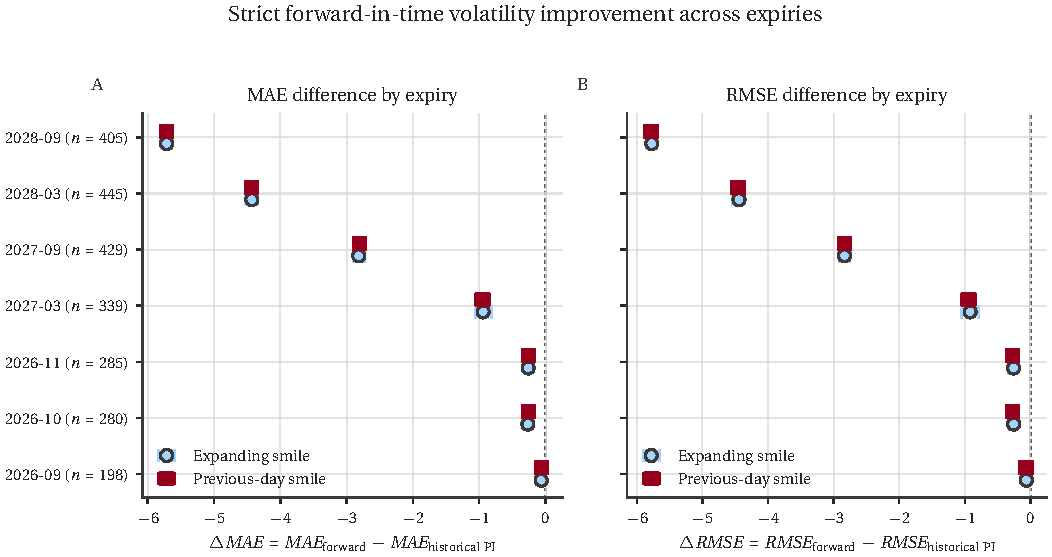
\includegraphics[width=\textwidth]{figures/publication/fig03_forward_q_cluster_bootstrap.pdf}
\caption{Strict forward-in-time pricing improvement across the seven admitted APO expiries. Points report the difference between each prior-date APO-smile error and the historical posterior-integrated baseline on the same holdouts; Panel A uses MAE and Panel B RMSE. Horizontal bars are 95\% percentile intervals from 100,000 valuation-date cluster bootstrap resamples, preserving dependence among contracts observed on the same market date. The dotted vertical line at zero is the no-difference benchmark: values to its left indicate lower error for the option-informed specification, whereas values to its right indicate worse performance relative to the historical-volatility baseline. Both the expanding and previous-day specifications use only implied-volatility observations dated strictly before each target date.}
\label{fig:forward_q_bootstrap}
\end{figure*}

The result is not driven by one expiry. Both prior-date specifications improve MAE and RMSE relative to the historical-volatility baseline in every admitted expiry. In the pooled panel, the expanding smile lowers MAE by 95.8\% and RMSE by 94.9\%, while the previous-day smile lowers MAE by 95.9\% and RMSE by 95.3\%. Mean pricing error moves from +2.4030 under the historical-volatility baseline to $-0.0697$ and $-0.0352$, respectively. The sign change relative to the short-dated October baseline reflects the maturity structure above: a long-window historical volatility near 0.416 is below the effective APO level for some 2026 expiries but substantially above the effective level embedded in the 2027--2028 marks.

A stronger benchmark asks whether this difference is merely a recency or historical-forecasting effect. Table~\ref{tab:recent_history_persistence} Panel A evaluates four pre-specified recent historical estimators and a horizon-matched Gaussian GARCH(1,1) forecast on the exact same 2,381 holdouts. None of these evaluated historical comparators reproduces the option-informed performance. The best pooled recent-history rule is the 63-return estimator, with MAE 4.5201 and RMSE 5.6465, both worse than the long-window historical PI benchmark. The more structured GARCH benchmark updates conditional variance at the target date, forecasts variance over each remaining fixing horizon, and then matches the implied arithmetic-average variance with one constant annualized volatility; its pooled MAE/RMSE are 2.6730/3.4441, close to the long-window historical PI values of 2.6187/3.4090. These specific recent-history and dynamic historical benchmarks therefore do not account for the observed option-informed advantage; the experiment does not rule out all possible historical forecasting models.

\begin{table*}[t]
\centering
\caption{Historical-volatility and persistence benchmarks for the strict-forward APO experiment. Panel A uses the same 2,381 contract-date holdouts and 15 target dates as the main forward comparison and includes both backward-looking scalar estimators and a horizon-matched Gaussian GARCH(1,1) forecast. Panel B restricts all methods to the 2,366 contract-dates for which the same contract has a strictly prior implied volatility. Historical PI is the canonical Monte Carlo posterior-integrated baseline; scalar historical, GARCH, and option-implied inputs are repriced with the deterministic Curran engine. All option-informed inputs are dated strictly before the target date.}\label{tab:recent_history_persistence}

\textit{Panel A: historical-volatility benchmarks on the exact forward holdouts}\\[2pt]
\begin{tabular}{lrrrr}
\toprule
Volatility input & $N$ & Dates & MAE & RMSE\\
\midrule
Long-window historical PI & 2,381 & 15 & 2.6187 & 3.4090\\
Rolling 252 returns & 2,381 & 15 & 5.2183 & 6.3933\\
Rolling 126 returns & 2,381 & 15 & 8.3419 & 9.7846\\
Rolling 63 returns & 2,381 & 15 & 4.5201 & 5.6465\\
EWMA, half-life 63 days & 2,381 & 15 & 5.6616 & 6.8824\\
Horizon-matched GARCH(1,1) & 2,381 & 15 & 2.6730 & 3.4441\\
Prior-date APO expanding smile & 2,381 & 15 & 0.1088 & 0.1725\\
Prior-date APO previous-day smile & 2,381 & 15 & 0.1075 & 0.1594\\
\bottomrule
\end{tabular}

\vspace{5pt}
\textit{Panel B: contract-level persistence on exact common rows}\\[2pt]
\begin{tabular}{lrrrr}
\toprule
Volatility input & $N$ & Dates & MAE & RMSE\\
\midrule
Historical PI & 2,366 & 15 & 2.6279 & 3.4173\\
Prior-contract IV carry & 2,366 & 15 & 0.0992 & 0.1403\\
Previous-day fitted APO smile & 2,366 & 15 & 0.1074 & 0.1594\\
\bottomrule
\end{tabular}
\end{table*}

Panel B separates option information from cross-sectional fitting flexibility. A same-contract persistence rule carries the latest strictly prior APO implied volatility forward and reprices the contract using the target-date futures curve, discount factor, realized fixings, and remaining fixing schedule. It is available for 2,366 of the 2,381 holdouts. On those exact common rows, prior-contract IV carry has MAE 0.0992 and RMSE 0.1403, compared with 0.1074 and 0.1594 for the fitted previous-day smile. This is a descriptive pooled ranking rather than evidence of general or statistically significant superiority of carry over the fitted smile. Its role is narrower: the large improvement over the historical-volatility inputs does not require flexible cross-sectional smoothing.

Section~\ref{sec:robustness} reconstructs the physical return history contract by contract from official first-nearby CL settlements. On these exact 2,381 holdouts, the reconstructed historical baseline has MAE 2.6468 and RMSE 3.4451 rather than 2.6187 and 3.4090. The option-informed errors are unchanged, so the central forward comparison is insensitive to the continuous-contract return proxy.

Liquidity restrictions preserve the central result. The 62 positive-volume holdouts span 13 valuation-date clusters: historical PI has MAE 1.6340 and RMSE 2.3391, compared with 0.1003 and 0.1358 for the expanding smile and 0.1084 and 0.1333 for the previous-day smile. At open interest of at least 100, the corresponding forward MAEs are approximately 0.106--0.107 versus 1.990 for the historical baseline. The long-dated positive-volume counts remain sparse within individual expiries, however, so the strongest statement concerns the pooled transaction-active sample and the much denser open-interest-filtered cross sections.

The forward result changes the interpretation of the empirical exercise. The observed pricing errors are not primarily a consequence of failing to integrate the historical volatility posterior. The evaluated recent-history rules do not reproduce the option-informed performance, and the horizon-matched GARCH experiment shows that adding conditional heteroskedasticity and maturity-specific variance forecasting does not materially narrow the pooled gap. GARCH improves RMSE relative to the long-window historical baseline for October 2026 and September 2028, but remains far from the option-informed specifications at every expiry. The persistence benchmark adds a separate point: on the common sample, carrying a contract's own prior implied volatility yields lower pooled error than the fitted smile, so the historical-versus-option-informed improvement does not depend on cross-sectional smile flexibility.

This comparison does not eliminate a role for Bayesian parameter uncertainty. The mechanism map shows where the posterior-integration correction can become appreciable. In the observed holdouts, however, changing from historical volatility inputs to recent option-implied states changes pricing errors far more than integrating the relatively concentrated historical posterior through the local pricing map. This remains an empirical benchmark comparison rather than a pure structural decomposition, because option-implied and historical inputs differ in information source and may embed risk premia, omitted dynamics, and market-marking effects.

\subsection{Independent vanilla-WTI validation}\label{sec:external_lo_results}

The strict APO-forward experiment leaves one important identification concern: its risk-neutral state is inferred from the same option family later used as the pricing target. The vanilla-WTI experiment addresses that concern by constructing the volatility surface only from prior-date LO and CL settlements. The final strike expansion to 70--120 places 253 of the 280 matched October contract-dates inside the observed prior LO moneyness support, compared with only 60 observations under the initial narrow strike pilot. Only 50 of 620 external-surface prediction rows require any support clipping.

Table~\ref{tab:external_lo} reports the exact no-clipping comparison. Historical-volatility posterior integration has MAE/RMSE 0.4464/0.5562 with Yahoo \texttt{CL=F} and 0.4362/0.5466 with the reconstructed first-nearby history. The external previous-day LO surface lowers these errors to 0.1559/0.2599, while the expanding LO surface gives 0.1604/0.2858. The corresponding prior-date APO smiles are 0.1676/0.2686 and 0.1612/0.2912. Thus an independently observed vanilla-WTI risk-neutral surface reproduces the large pricing improvement previously obtained from the APO market itself, and that comparison is insensitive to the historical return-source construction.

\begin{table*}[t]
\centering
\caption{Independent vanilla-WTI validation on the exact common-support sample. All methods are evaluated on the same 253 October-2026 APO contract-dates over 10 valuation dates. The historical rows are canonical Monte Carlo posterior-integrated prices and differ only in the physical-return source: Yahoo \texttt{CL=F} versus the contract-reconstructed first-nearby CL settlement series. External LO and prior-date APO surface rows are deterministic Curran repricings; external LO surfaces use only vanilla observations dated strictly before the APO target date.}\label{tab:external_lo}
\begin{tabular}{lrrr}
\toprule
Method & $N$ & MAE & RMSE\\
\midrule
Historical PI, Yahoo \texttt{CL=F} & 253 & 0.4464 & 0.5562\\
Historical PI, reconstructed first-nearby & 253 & 0.4362 & 0.5466\\
External LO surface, previous day & 253 & 0.1559 & 0.2599\\
External LO surface, expanding & 253 & 0.1604 & 0.2858\\
Prior-date APO smile, previous day & 253 & 0.1676 & 0.2686\\
Prior-date APO smile, expanding & 253 & 0.1612 & 0.2912\\
\bottomrule
\end{tabular}
\end{table*}

The valuation-date cluster bootstrap confirms that the external improvement over historical volatility is not driven by treating same-day contracts as independent. For the previous-day LO surface, the MAE difference relative to historical PI is $-0.2905$, with a 95\% interval of $[-0.3439,-0.2333]$, and the RMSE difference is $-0.2963$, with interval $[-0.3503,-0.2580]$. The expanding LO surface produces corresponding differences of $-0.2860$ and $-0.2704$, again with intervals entirely below zero.

The external and APO-implied surfaces are much closer to one another. Previous-day LO has an MAE difference of $-0.0117$ relative to the previous-day APO smile, with a 95\% interval of $[-0.0251,-0.0001]$; its RMSE difference is $-0.0087$, with interval $[-0.0149,0.0002]$. For the expanding specifications, both the MAE and RMSE intervals include zero. These results do not establish global superiority of vanilla LO over APO-implied volatility. Their more important implication is that the pricing gain associated with an option-informed risk-neutral state survives when the volatility source is moved outside the APO family.

The independent LO evidence leads to the same narrower comparison: the point-price effect of integrating the maintained historical-volatility posterior is much smaller than the pricing difference obtained from recent option-informed volatility inputs. This statement is supported by both within-family forward APO evidence and cross-instrument LO evidence. Bayesian integration propagates uncertainty conditional on the maintained model; it does not by itself resolve a volatility input that is empirically misaligned with option settlements.


\section{Robustness and limitations}\label{sec:robustness}

The main text keeps only the robustness evidence needed to interpret the three central findings. Full sampler settings, alternative-window results, posterior calibration, numerical audits, tree-refinement diagnostics, and extended liquidity tables are preserved in the online supplement.

\subsection{Historical-model and data robustness}

The historical-versus-option-informed comparison is not driven by one particular historical estimator. Table~\ref{tab:recent_history_persistence} shows that the evaluated rolling-window and EWMA rules do not reproduce the prior option-implied performance, while the horizon-matched GARCH benchmark remains close to the long-window historical baseline. The GARCH result is useful because it allows conditional heteroskedasticity and maturity-specific variance forecasting rather than treating historical volatility as a single static estimate. Its failure to close the pooled gap narrows the interpretation to the tested historical models without implying that every possible historical forecast has been ruled out.

Other changes to the physical-measure specification have similarly modest effects on the main hierarchy. Replacing Gaussian innovations with standardized Student-\(t\) returns modestly improves historical-volatility pricing but leaves the PI--PM correction small relative to the remaining pricing error. Reconstructing the physical return history contract by contract from first-nearby CL settlements yields a volatility posterior very close to the Yahoo \texttt{CL=F} baseline and leaves the forward comparison essentially unchanged. Prior and estimation-window sensitivity show that, once the long historical likelihood is informative, reasonable prior changes have little effect; shorter windows matter more because they sample different volatility regimes.

A posterior-RMS plug-in provides a separate scalar check. Repricing the posterior mean and posterior RMS with the same deterministic Curran engine changes pooled pricing error only slightly. This comparison is intentionally common-engine: it isolates the scalar posterior summary and should not be confused with the main Monte Carlo posterior-integrated historical benchmark.

\subsection{Numerical and statistical validation}\label{sec:numerical_robustness}

The empirical PI--PM correction is small enough that numerical error must be ruled out directly. High-precision pseudo-random Monte Carlo, independently scrambled Sobol calculations, and Curran conditioning agree on the PI--PM difference to a scale well below the observed empirical gaps. The conclusion that posterior integration adds little to the October point-price mean is therefore not an artifact of simulation noise or one particular pricing engine.

The posterior implementation is checked separately through simulation-based calibration. Prior-predictive rank distributions and interval coverage are close to their nominal targets across the tested sample sizes. For the external LO inversion, an 80/160/320-step CRR refinement audit shows practical stability at the production 160-step choice, while a separate surface-shape audit finds finite positive fitted volatilities and smooth behavior inside observed prior support. These diagnostics support numerical implementation; they are not presented as proofs of an exact infinite-tree limit or of a globally arbitrage-free fitted surface.

\subsection{Liquidity, persistence, and external transfer}

Dependence across contracts is handled by resampling valuation dates rather than individual option rows. Cluster-bootstrap comparisons preserve the large separation between prior option-informed specifications and the historical baseline. The same direction also appears in the positive-volume pool and across open-interest restrictions, although transaction-active observations remain sparse in the longest-dated expiries. The empirical claims therefore concern available end-of-day market marks rather than a dense transaction-price panel.

The same-contract persistence experiment provides a distinct interpretation check. On the exact common sample, carrying each contract's latest strictly prior implied volatility gives lower pooled error than the fitted previous-day smile. This is a descriptive ranking, not evidence that IV carry is generally superior. Its role is narrower: the historical-versus-option-informed improvement does not require flexible cross-sectional smile fitting.

The external LO result is also robust to the scalar transfer rule. Replacing the primary fixing-count RMS mapping with a scalar chosen to match the unresolved arithmetic-average variance changes the external pricing errors only slightly. Thus the cross-instrument conclusion does not depend on treating the primary RMS mapping as an exact variance identity.

\subsection{Limits of interpretation}

The forward APO experiment spans seven expiries but only 15 distinct target dates, and the external common-support experiment spans 10 target dates. Multiple contracts on one date expand the cross-section but do not create additional independent market histories. Date-cluster resampling preserves contemporaneous dependence but does not remove serial dependence across adjacent dates.

The pricing model is also deliberately parsimonious. A multi-factor futures curve, stochastic volatility, jumps, stochastic convenience yield, or richer interest-rate treatment could improve absolute pricing fit and would introduce additional uncertain parameters. The present evidence does not identify a pure structural \(\mathbb P\)--\(\mathbb Q\) volatility wedge: option-implied states can absorb risk premia, omitted dynamics, liquidity, and settlement-marking effects. The paper's narrower conclusion is conditional on the maintained pricing map and the historical benchmarks actually evaluated.

\section{Conclusion}\label{sec:conclusion}

This paper isolates a narrow Bayesian pricing question: how much does integrating uncertainty in historically estimated volatility change a WTI Average Price Option value relative to plugging in the posterior mean? The answer is governed by posterior dispersion and pricing curvature. Synthetic experiments confirm this mechanism and show that posterior integration can become economically relevant when information is weak and the pricing map is sufficiently curved.

The observed WTI sample lies in a different region. Posterior-integrated and posterior-mean point values are very close, yet the posterior distribution of theoretical prices remains materially wider. The distinction matters: a small \(C_{PI}-C_{PM}\) is a statement about nonlinear averaging of the posterior, not about the absence of parameter-induced price uncertainty.

The larger empirical margin is the volatility information supplied to the pricing map. Across the tested forward benchmarks, prior option-implied volatility states predict APO settlements much better than the historical-volatility inputs. That finding survives recent-window, EWMA, and horizon-matched GARCH comparisons; it does not require flexible smile fitting; and it remains visible when the volatility source is moved to an independent vanilla-WTI option market. These results support an option-informed versus tested-historical comparison, not a pure structural decomposition between physical and risk-neutral volatility.

The contribution is therefore diagnostic rather than a new option-pricing theory. Posterior integration matters when dispersion meets curvature, but in this sample improving the volatility information is much more consequential for point pricing than more exact integration of the historical-volatility posterior. The evidence is limited by the small number of distinct market dates, uneven liquidity, and the maintained one-factor pricing model. Richer commodity dynamics can be studied from this benchmark without conflating model enrichment with the narrower effect of Bayesian posterior integration.


\bmsection*{Data availability}
The APO and CL histories used in the empirical application were obtained through a commercial Barchart subscription. The independent vanilla-WTI validation uses CME/NYMEX LO option and CL futures statistics accessed through Databento. Redistribution of raw proprietary market-data files is not assumed to be permitted. The public repository therefore prioritizes code, query metadata, schemas, provenance records, diagnostics, hashes, and derived results consistent with the applicable data licenses.

\bmsection*{Code availability}
The research code is organized as an installable Python package, \texttt{bayesian\_asian\_options}, with documented APIs, tests, deterministic seeds, reproducible experiment entry points, and committed derived results. The public repository is \url{https://github.com/heri-espino/Bayesian-Uncertainty-in-WTI-APOs}. The submitted manuscript and figures will be tied to the exact Git commit used for the submission build; that commit will be preserved as the versioned submission snapshot.

\bmsection*{Conflict of interest}
The author declares no conflict of interest.

\bmsection*{Acknowledgments}
To be completed before submission.

\bibliography{references}

\end{document}
